
% This LaTeX was auto-generated from an M-file by MATLAB.
% To make changes, update the M-file and republish this document.

%%% \documentclass{article}
%%% \usepackage{graphicx}
%%% \usepackage{color}

%%% \sloppy
%%% \definecolor{lightgray}{gray}{0.5}
\setlength{\parindent}{0pt}

%%% \begin{document}

    
    
\subsection*{Allan Overlapping Deviation}

\begin{par}
Example for algorithm OADEV.
\end{par} \vspace{1em}
\begin{par}
OADEV is an algorithm to compute the overlapping Allan deviation for a set of time-domain frequency data.
\end{par} \vspace{1em}
\begin{par}
See also W. J. Riley, "The Calculation of Time Domain Frequency Stability". Implementation: M. A. Hopcroft, \verb"mhopeng@gmail.com", Matlab Central.'
\end{par} \vspace{1em}

\subsubsection*{Contents}

\begin{itemize}
\setlength{\itemsep}{-1ex}
   \item Generate sample data
   \item Call algorithm
   \item Display results
\end{itemize}


\subsubsection*{Generate sample data}

\begin{lstlisting}[style=mcode]
DI = [];
%!demo
%ysin=2.*sin(2.*pi.*1/300.*[1:1:1e3]);
%! [x y s errors]=adev(1, ysin, 1, 'best averaging time is 300 s, i.e. cca one sine period');
% A random numbers with normal probability distribution function will be generated into data input |DI.y.v|.
DI.y.v = 1.5 + 3.*randn(1, 1e3);
% Next a drift is added:
DI.y.v = DI.y.v + [1:1:1e3]./100;
% Lets suppose a sampling frequency is 1 Hz:
DI.fs.v = 1;
% Let the algorithm generate all possible tau values automatically:
DI.tau.v = [];
\end{lstlisting}


\subsubsection*{Call algorithm}

\begin{par}
Use QWTB to apply algorithm \lstinline{OADEV} to data \lstinline{DI}.
\end{par} \vspace{1em}
\begin{lstlisting}[style=mcode]
DO = qwtb('OADEV', DI);
\end{lstlisting}

        \begin{lstlisting}[style=output]
QWTB: no uncertainty calculation
\end{lstlisting} \color{black}
    

\subsubsection*{Display results}

\begin{par}
Log log figure is the best to see allan deviation results:
\end{par} \vspace{1em}
\begin{lstlisting}[style=mcode]
figure; hold on
loglog(DO.tau.v, DO.oadev.v, '-b')
loglog(DO.tau.v, DO.oadev.v + DO.oadev.u, '-k')
loglog(DO.tau.v, DO.oadev.v - DO.oadev.u, '-k')
xlabel('\tau (sec)');
ylabel('\sigma_y(\tau)');
title(['period = ' num2str(DI.fs.v)]);
grid('on'); hold off
\end{lstlisting}

\begin{center}
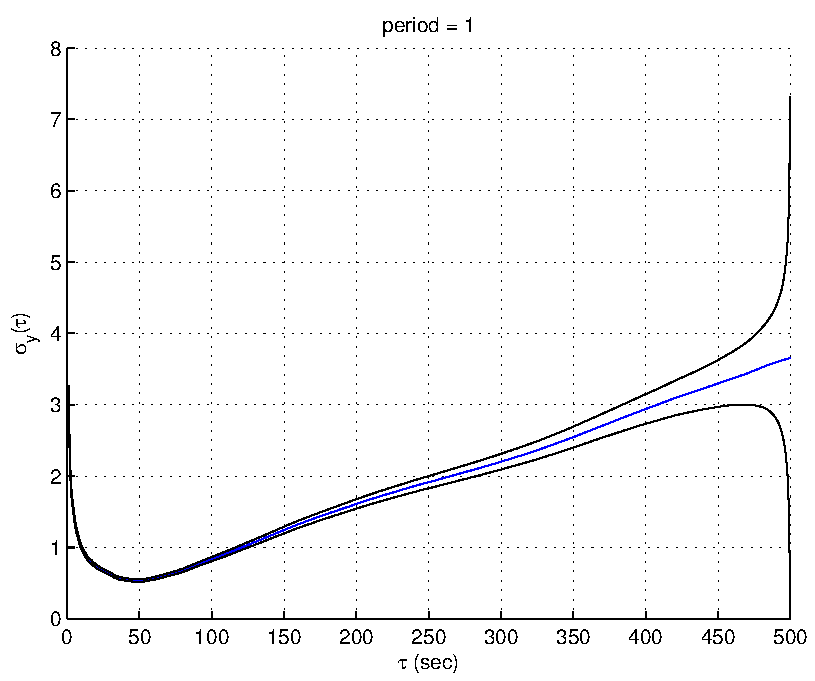
\includegraphics[width=0.7\textwidth]{algs_examples_published/OADEV_alg_example_01.pdf}
\end{center}



%%% \end{document}
    
